\documentclass{article}

\usepackage{amsfonts,relsize,amsmath,amssymb,systeme}
\usepackage{listings}

\usepackage{hyperref}

\usepackage{graphicx}
\graphicspath{ {./images/} }

\usepackage[T1]{fontenc}
\usepackage[polish]{babel}
\usepackage[utf8]{inputenc}
\usepackage{lmodern}
\selectlanguage{polish}
\author{Autor: Zbigniew Królikowski
\\\\\\\\}
\title{ Algorytmy dla Problemów Trudnych Obliczeniowo.\\
Rozwiązanie zadania: \textbf{Potęga hetmanów}
Informatyka 2015/16}


\begin{document}
\maketitle


\vfill

\paragraph{Prowadzący: dr hab. inż. Piotr Faliszewski
\\\\\\\\
}

\newpage

\tableofcontents

\newpage

\section{Reprezentacja problemu}

Plansza została przedstawiona jako \textbf{graf nieskierowany}, w którym każdy węzeł połączony jest z innymi co najwyżej 8 krawędziami.

\subsection{Zapis wartości hetmanów}

W celach uproszczenia obliczeń wartości są reprezentowane jako wykładniki liczby 2 \textbf{przesunięte} jednak o 1 w górę, tak aby prawidłowo oddać arytmetykę.

\section{Wstępne obserwacje}

\begin{figure}[!ht]
  \centering
      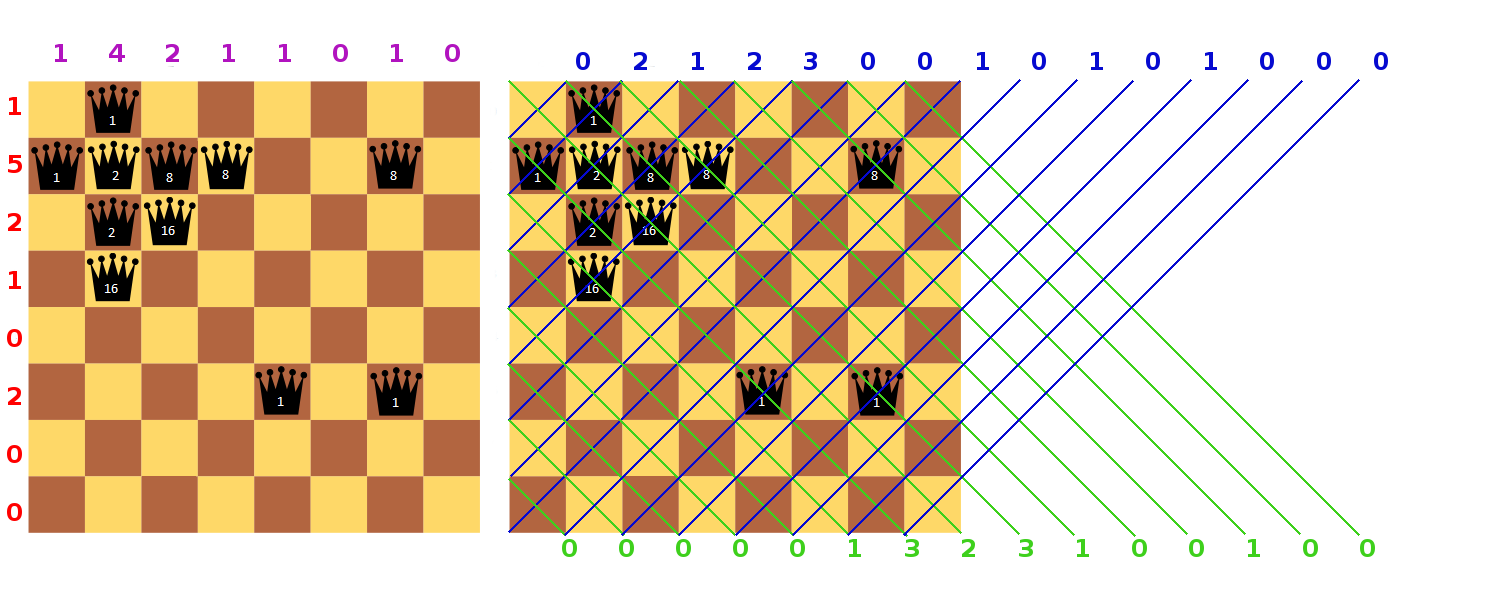
\includegraphics[scale=0.3]{obs1.png}
  \caption{Przykładowy obszar z dwoma rodzajami pól.}
\end{figure}

\end{document}
